\section{Main Algorithm}\label{sec:algo}

To address these problems, we extended \learnpads{} to work
incrementally.  
\figref{fig:overview} illustrates the overall process.
Given a candidate description \cd{D}, the new algorithm uses \cd{D} to parse
the records in the data source.  
It discards records that parse successfully, since these records are
already covered by \cd{D}, but it collects records that fail to parse.
Specifically, if a portion of a record fails to parse,
that failure will be detected at a particular node in \cd{D}.
These failed portions are collected
in an aggregation data structure \cd{A} that mirrors the the structure
of \cd{D}. When the algorithm accumulates $M$ such records, where $M$ is a
parameter of the algorithm, it transforms \cd{D} to accommodate the places 
where differences were found (\ie, by introducing options where a piece of
data was missing or unions where a new type of data was discovered).
It then uses the original \learnpads{} algorithm to infer descriptions
for the aggregated portions of bad data, and merge these new
sub-descriptions into the transformed description to produce a new,
refined description \cd{D'}. This refined
description subsumes \cd{D} and describes the $M$
new records.  In addition, the algorithm attempts to preserve as much
of the structure of \cd{D} as possible, so users supplying initial
descriptions can recognize the resulting descriptions. 
The algorithm then makes \cd{D'}
the new candidate description and repeats the process until it
has consumed all the input data. We call the main loop in 
\figref{fig:overview} the {\em incremental learning step}.
The initial description \cd{D} can either be supplied by a user or it
can be inferred automatically by applying the original algorithm to
$N$ records selected from the data source, where $N$ is another
parameter.  
%Currently, the system selects a mix of $N/3$ consecutive lines
%taken from the beginning, middle, and end of the data source. 

\cut{%%%%%%%%%%%%%%%%
Intuitively, the incremental learning step works by attempting to
parse each of the $M$ records according to the current description
\cd{D}.  It discards the portions of each record that parse correctly.
If a portion fails to parse, that failure will be detected at a
particular node in the description \cd{D}. It collects these failed
portions in an aggregation data structure \cd{A} that mirrors the
structure of \cd{D}.  After thus aggregating all the failures in the $M$
records, the algorithm transforms \cd{D} to accommodate the places where
differences were found (\ie, by introducing options where a piece of
data was missing or unions where a new type of data was discovered).
It then uses the original \learnpads{} algorithm to infer descriptions
for the aggregated portions of bad data. 
}%%%%%%%%%% end of cut

In the following, we present the algorithm in more detail.

\cut{
Intuitively, the incremental learning algorithm takes an initial
description as input, divides the new data into manageable
chunks, and iteratively merges descriptions of these chunks into the
current description.
\figref{fig:overview} illustrates a high level schematic of this
algorithm. A large or streaming data source is input 
to the system in batches. Each batch of data contains $M$ 
records, where $M$ is a parameter of the framework.
%%The state of the system is determined by the current data
%%description which is subject to change as new data streams into the system. 
The initial description
can be supplied by user, or learned from the first batch of the input
data. At each iteration, the system generates a filter program from
the current data description.  This program parses the incoming batch of data
into an aggregated data structure similar to the parse tree of the description.
In this process, the filter program collects ``bad data'' which does not
conform to the current description. The system then invokes the original
\learnpads{} algorithm to learn ``sub-descriptions'' from the bad data, and
merges these sub-descriptions into the current data description to produce
a new description for the next iteration. 
}
\begin{figure}[t]
\centering
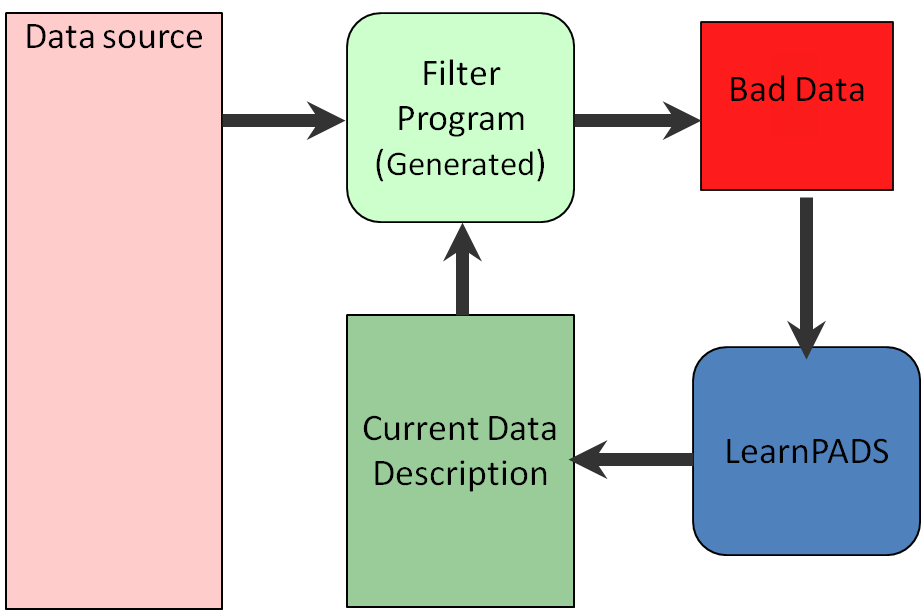
\includegraphics[width=0.8\columnwidth]{overview}
%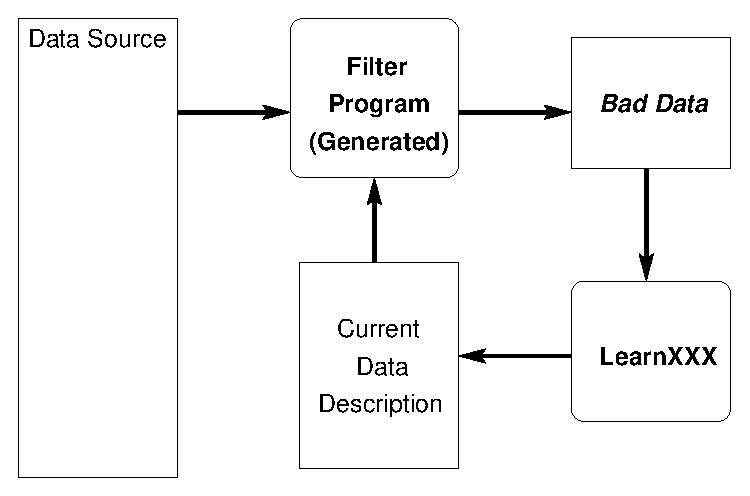
\epsfig{file=overview.eps,width=0.9\columnwidth}
\caption{An Overview of the Incremental Learning Framework}
\label{fig:overview}
\vskip -2ex
\end{figure}

%To address these problems, 
%we extended \learnpads{} to work incrementally.  
%Given a candidate description \cd{D}, the new algorithm uses \cd{D} to parse
%the records in the data source.  
%It discards records that parse successfully, since these records are
%already covered by \cd{D}, but it collects records that fail to parse.
%When the algorithm accumulates $M$ such records, where $M$ is a
%parameter of the algorithm, it invokes the incremental learning step,
%described below, to produce a refined description \cd{D'}.  This refined
%description subsumes \cd{D} and describes the $M$
%new records.  In addition, the algorithm attempts to preserve as much
%of the structure of \cd{D} as possible, so users supplying initial
%descriptions can recognize the resulting descriptions. 
%The algorithm then takes \cd{D'}
%to be the new candidate description and repeats the process until it
%has consumed all the input data.
%The initial description \cd{D} can either be supplied by a user or it
%can be inferred automatically by applying the original algorithm to
%$N$ records selected from the data source, where $N$ is another
%parameter.  
%Currently, the system selects a mix of $N/3$ consecutive lines
%taken from the beginning, middle, and end of the data source. 

\subsection{Preliminaries}

\begin{figure}[t]
{\small 
\begin{code}
\kw{Basic notation}:
c            (a string character)	
s1.s2        (concatenation of strings)
first(s)     (first character of s)
prefix(s)    (set of prefixes of s) 
sprefix(s)   (set of strict prefixes of s)
len(s)       (length of s)
\end{code}
\begin{code}
\kw{Descriptions}:
Base ::= Pint | PstringME(re) | PstringFW(e)
\end{code}
\begin{code}
D ::=   
  Base               (Base token)
| Sync s             (Synchronizing token) 
| Pair (x:D1, D2)    (Pair with dependency)
| Union (D1, D2)     (Union)
| Array(D, s, t)     (Array)
| Option D           (Option)
\end{code}
\begin{code}
\kw{Data representation}:
BaseR ::= Str s | Int i | Error
\end{code}
\begin{code}
SyncR ::= Good | Fail | Recovered s 
\end{code}
\begin{code}
R ::=
  BaseR
| SyncR
| PairR (R1, R2)
| Union1R R | Union2R R 
| ArrayR (R list, SyncR list, SyncR)
| OptionR (R option)
\end{code}
\begin{code}
\kw{Aggregation structure}:
A :: = 
  BaseA Base
| SyncA s
| PairA(A1, A2)
| UnionA(Al, Ar)
| ArrayA (A_elem, A_sep, A_term)
| OptionA A
| Opt A
| Learn [s]
\end{code}
}
\vskip -2ex
\caption{Preliminary data structures used in incremental inference}
\label{fig:data-structures}\vskip -2ex
\end{figure}

\cut{%%%%%%%%%%%%%%%%%%%%%%%%%%%%%%%%%%%%%%%%%
Intuitively, the incremental learning step works by attempting to
parse each of the $M$ records according to the current description
\cd{D}.  It discards the portions of each record that parse correctly.
If a portion fails to parse, that failure will be detected at a
particular node in the description \cd{D}. It collects these failed
portions in an aggregation data structure \cd{A} that mirrors the
structure of \cd{D}.  After thus aggregating all the failures in the $M$
records, the algorithm transforms \cd{D} to accommodate the places where
differences were found (\ie, by introducing options where a piece of
data was missing or unions where a new type of data was discovered).
It then uses the original \learnpads{} algorithm to infer descriptions
for the aggregated portions of bad data. 
}%%%%%%%%%%%%%%%%%%%%%%%%%%%%%%%%%%%%%%%%%%%%%%%%%%%%

\figref{fig:data-structures} defines
the data structures for descriptions \cd{D}, data
representations \cd{R}, and aggregate structures \cd{A}.
Some data types, such as the switched union, are omitted for the succinctness
of the presentation.
In these definitions,  variable \cd{re} ranges over regular expressions,
\cd{e} over host language expressions,
\cd{s} and \cd{t} over strings, and \cd{i} over integers.
%A value with type \cd{D} is the abstract syntax tree of \pads{}
%description: this description is what we want to learn.  
For simplicity of presentation, we assume just three base types: 
integers, strings that match a regular expression and strings with a
fixed width specified by an expression. Synchronizing
tokens, or {\em sync tokens} for short, correspond to string literals
in \pads{} descriptions.  Such tokens, which are often
white spaces or punctuation,
serve as delimiters in the data and are useful for detecting
errors. The binary dependent pairs \cd{Pair (x:D1, D2)} are
a simplification of \pads{} more general \kw{Pstruct}s. 
The variable \cd{x} refers to the data parsed by \cd{D1}
and may be used in \cd{D2}. The union \cd{Union (D1, D2)}
provides a choice between descriptions \cd{D1} and \cd{D2}.
An array description
\cd{Array(D, s, t)} has an element type described by \cd{D}, a separator
string \cd{s} that appears between array elements, and a
terminator string \cd{t}. Finally, \cd{Option D} indicates \cd{D} is 
optional.  To resolve ambiguities, unions are
biased towards their first element, arrays are biased towards a longest match
semantics and options are biased towards matching as opposed to not matching.

A term \cd{R} is a parse tree obtained from parsing 
data using a description \cd{D}.  Parsing a base type can result in a
string, an integer or an error.  Parsing a sync token
\cd{Sync s} can give three different results: \cd{Good}, meaning the
parser found \cd{s} at the beginning of the input; \cd{Fail}, meaning
\cd{s} is not a substring of the current input; or \cd{Recovered s'},
meaning \cd{s} is not found at the beginning of the input, but
can be {\em recovered} after ``skipping'' string \cd{s'}.  The parse
of a pair is a pair of representations, and the parse of a union is
either the parse of the first branch or the parse of the second
branch. The parse of an option is either the parse of its body or  empty.
The parse of an array includes a list of parses for the
element type, a list of parses for the separator and a parse for the
terminator which appears at the end of the array.

An aggregation structure accumulates the set of currently
unparseable data fragments whose form must be learned
for inclusion in the grammar.
The aggregation structure mirrors the structure of the description \cd{D} 
with two additional nodes: an \cd{Opt} node and a \cd{Learn} node. 
%Note the difference between {\tt Opt} nodes and {\tt OptionA} nodes. The latter 
%just corresponds to the description {\tt Option D}. 
The \cd{Learn} nodes accumulate extra data whose structure must be learned.
The \cd{Opt} nodes do the opposite: they mark were data were missing.  
An invariant
of the aggregation structure is that
newly inserted \cd{Opt} nodes always wrap either a \cd{BaseA} or 
a \cd{SyncA} node.

%Once the system infers a description for this accumulated data, it
%splices in the new description in place of the \cd{Learn} node.

\subsection{Incremental Learning Step}
\begin{figure}[t]
\begin{codebox}
incremental_step(D, xs) =
  As = [\kw{init_aggregate}(D)];
  foreach x in xs \{
    Rs = \kw{parse}(D, x);
    As' = [];
    foreach R in Rs \{
      foreach A in As \{
        A' = \kw{aggregate}(A, R); 
        As' = A' :: As'
      \}
    \}
    As = As'
  \} 
  best_a = \kw{select_best}(As);
  D' = \kw{update_desc}(D, best_A);  
  return D'
\end{codebox}
\caption{Pseudo-code for the incremental learning step}
\label{fig:inc-learning}
\vskip -2ex
\end{figure}

\figref{fig:inc-learning} gives pseudo-code for the {\em incremental
  learning step}.  The input  is the current description
\cd{D} and a batch of data records \cd{xs}.  The \kw{init\_aggregate}
function initializes an empty aggregate according to description
\cd{D}.  During parsing, the algorithm iteratively updates a list of
possible aggregates \cd{As}, seeded with the initial aggregate of
\cd{D}.  For each data record \cd{x}, the algorithm uses the
\kw{parse} function to produce a list \cd{Rs} of possible parses.  It
then calls the \kw{aggregate} function to merge each parse \cd{R} in
the current list of parses with each aggregate \cd{A} in the current
list of aggregates.  (We use `\cd{::}' to denote prepending an element
onto the front of a list.) Note that the potentially large number of parses
and the growing list of aggregates in the
inner loop are the performance bottleneck. 
We will show in Section \ref{sec:opt}
some strategies to alleviate this complexity.  

When the system finishes parsing all the
input data, the algorithm uses the \kw{select\_best} function to
select the best aggregate from the list of candidate aggregates
\cd{As}.  The \kw{select\_best} function counts the total number of
\cd{Opt} and \cd{Learn} nodes in each of the aggregates, and returns
the one with the smallest number.
The idea is that the aggregate with the smallest number of added nodes is 
more likely to represent a description
that is the close to the original description. 

Finally, the \kw{update\_desc} function uses the structure of the best
aggregate to update the previous description \cd{D} to produce the new
current description \cd{D'}.  The \kw{update\_desc} function works by
doing two things.
First, it converts the aggregate structure back to a \pads{} description
with \cd{Opt} nodes translated to \cd{Poption} types. In addition,
it invokes the \learnpads{} format inference
algorithm to learn a sub-description for the data collected 
at each of the \cd{Learn} nodes
and replaces these \cd{Learn} nodes with these new sub-descriptions. 
Second, it uses rewriting
rules to improve the overall description.
%We will discuss these rewriting rules in more
%detail in \secref{sec:imp}.

\begin{figure}[t]
%\begin{center}
{\small
\begin{code}
\cdmath\small
\kw{Base}:
(Int (atoi s), m) $\in$ L(Pint,E,s,s')
  if re = (+|-)?[0-9]+
  and s $\in$ L(re) 
  and s'' $\in$ prefix(s') and s.s'' $\not\in$ L(re)
  and m = (0,1,0,len(s))
(Error, (1,0,0,0)) $\in$ L(Pint,E,"",s'),
  if x $\in$ prefix(s') then x $\not\in$ L((+|-)?[0-9]+) 
(Str s, m) $\in$ L(PstringME(re),E,s,s'),
  if s $\in$ L(re) 
  and s'' $\in$ prefix(s') and s.s'' $\not\in$ L(re) 
  and m = (0,1,0,len(s)) 
(Error, (1,0,0,0)) $\in$ L(PstringME(re),E,"",s'), 
  if x $\in$ prefix(s') then x $\not\in$ L(re)
(Str s, m) $\in$ L(PstringFW(e),E,s,s') 
  if E(e) = Int k and k >= 0
  and s = c1...ck and m = (0,1,0,k)
(Error, (1,0,0,0)) $\in$ L(PstringFW(e),E,"",s') 
  if E(e) $\ne$ Int k for any k > 0
(Error, (1,0,0,0)) $\in$ L(PstringFW(e),E,"",s') 
  if E(e) = Int k and k > 0 and len(s') < k
\mbox{}
\kw{Sync}:
(Good, (0,1,0,len(s))) $\in$ L(Sync(s),E,s,s')
(Recovered s1, m) $\in$ L(Sync(s2),E,s,s')
  if s = s1.s2 
  and s3.s2 $\not\in$ sprefix(s1.s2) for any s3
  and m = (1,0,len(s1),len(s2))
(Fail, (1,0,0,0)) $\in$ L(Sync(s),E,"",s')
  if s $\not\in$ prefix(s')
\mbox{}
\kw{Pair}:
(PairR (R1,R2), (m1 + m2)) 
        $\in$ L(Pair(x:D1, D2),E,s1.s2,s')
  if  (R1, m1) $\in$ L(D1,E,s1,s2.s')
  and (R2, m2) $\in$ L(D2,E[x $\arrow$ R1],s2,s')
\mbox{}
\kw{Union}:
(Union1R R, m) $\in$ L(Union(D1, D2),E,s,s')
  if (R, m) $\in$ L(D1, E, s, s')
(Union2R R, m) $\in$ L(Union(D1, D2),E,s,s')
  if (R, m) $\in$ L(D2, E, s, s')
\mbox{}
\kw{Main parse function}:
\kw{parse}(D, s) = \{R | (R, m) $\in$ L(D,$\epsilon$,s,"")\} 
\end{code}
%and for all (R',m') $\in$ L(D,.,s,""), m <= m'
}
\caption{Definition of \kw{parse} function (excerpts)}
\label{fig:parse-sem}
%\end{center}
\end{figure}

%% \mbox{}
%% \kw{Array}:
%%   (ArrayR([R1,...,Rn], [SyncR1,...,SyncR(n-1)], $SyncR_{term}$), m)
%%     $\in$ L(Array(D, $s_{sep}$, $s_{term}$), E, s, s'),
%%         if
%%         s = s1.$s_{sep}$.s2.$s_{sep}$...s(n-1).$s_{sep}$.sn,
%%         lookaheadfori = $s_{sep}$.s(i+1).....sn.s'
%%         lookaheadforsepi = s(i+1)....sn.s'
%%         s' = s1'.lookaheadforterm

%%         forall i $\in$ [1, n]:
%%           (Ri, mi) $\in$ L(D, E, si, lookaheadfori),
%%         forall i $\in$ [1, n-1]:
%%           (SyncRi, m(s,i)) $\in$ L(Sync($s_{sep}$), E, $s_{(sep,i)}$, lookaheadforsepi),

%%         ($SyncR_{term}$, $m_{term}$) $\in$ L(Sync($s_{term}$), E, s1', lookaheadforterm),
%%         m = $\sum_{i= 1}^{n} mi$ + $\sum_{i=1}^{n-1} m(s,i)$ + $m_{term}$
%% \mbox{}
%% \kw{Option}:
%% (OptionR (SOME R), m) $\in$ L(Option D, E, s, s')
%%   if (R, m) $\in$ L(D, E, s, s')
%% (OptionR (NONE), m) $\in$ L(Option D, E, "", s')
%%   if (R, m) $\in$ L(D, E, "", s')


\subsection{Parsing}
\label{sec:parse}
Our parser is a top-down recursive descent parser
that performs error detection and recovery using synchronizing tokens.
\figref{fig:parse-sem} describes the most important elements
of the parsing algorithm.  For simplicity and brevity, we
describe the algorithm abstractly
using a relation of the form 
${\texttt{(R,m)} \in \texttt{L(D,E,s,s')}}$.  This relation may be
read ``using description \cd{D} and operating within the environment \cd{E},
parsing the input \cd{I = s.s'} will consume input prefix \cd{s} and leave \cd{s'} as the residual input, 
returning the parse tree \cd{R} and correctness metric \cd{m}.''   
The environment \cd{E} is a mapping from variable names
\cd{x} to parse trees \cd{R}.  This environment stores the
binding of variables to parse trees that the \pads{} dependent
pair construct introduces.   We use the symbol `$\epsilon$' to denote the empty environment.

The {\em parse metric} \cd{m} measures the quality of a parse. It is a 
4-tuple: ($e$, $g$, $s$, $c$), where the $e$ is the number of tokens
with parse errors, $g$ is the number of tokens parsed correctly,
$s$ is the number of 
characters skipped during \cd{Sync} token recovery, 
and $c$ is the number of characters correctly parsed. 
To sum two parse metrics, we sum their components:
$(e_1, g_1, s_1, c_1) + (e_2, g_2, s_2, c_2) = 
(e_1 + e_2, g_1 + g_2, s_1 + s_2, c_1 + c_2)$.
We compare parse metrics by comparing the ratios of correctly
parsed characters against erroneous tokens and the estimated number of
skipped tokens.  We estimate the number of skipped tokens
by computing the
fraction of the number of skipped characters over the estimated token
length:
\begin{eqnarray*}
(e_1, g_1, s_1, c_1) &\ge& (e_2, g_2, s_2, c_2)~ \rm{iff} \\
\frac{c_1}{e_1+\frac{s_1}{\max((s_1+c_1)/(e_1+g_1), 1)}} &\ge& 
\frac{c_2}{e_2+\frac{s_2}{\max((s_2+c_2)/(e_2+g_2), 1)}} \\
\end{eqnarray*}

%%\subsection{Aggregation}
%% \begin{figure}[t]
%% \centering
%% \begin{code}
%% \cdmath
%% \kw{Opt}:
%%   Opt a + Error $\goto$ Opt a
%%   Opt a + b     $\goto$ Opt b::a
%% \mbox{}
%% \kw{a : [Base]}:
%%   a + Error $\goto$ Opt a
%%   a + b     $\goto$ b::a
%% \mbox{}
%% \kw{a : [Sync s]}: 
%%   a + Good $\goto$ Good :: a
%%   a + Fail $\goto$ Opt a
%%   a + Recovered s' $\goto$ (Opt(l [s'], Good :: a)
%% \mbox{}
%% \kw{Opt a : Opt [Sync s]}: 
%%   Opt a + Good $\goto$ Opt (Good :: a)
%%   Opt a + Fail $\goto$ Opt a
%%   Opt a + Recovered s' $\goto$ 
%%     (Opt (l [s]), Opt (Good :: a))
%% \mbox{}
%% \kw{(Opt(l Ss), a) : Opt L * [Sync s]}:
%%   (Opt(l Ss), a) + Good $\goto$ 
%%     (Opt(l Ss), Good :: a)
%%   (Opt(l Ss), Opt a) + Fail $\goto$ 
%%     (Opt(l Ss), Opt a)
%%   (Opt(l Ss), Opt a) + Recovered s' $\goto$ 
%%     (Opt(l s':: Ss), Opt Good :: a)
%% \mbox{}
%% \kw{Pair(x:D1, D2)}:
%%   PairA($a_1$, $a_2$) + PairR($r_1$, $r_2$) $\goto$ 
%%     PairA($a_1\prime$, $a_2\prime$),
%%     if  $a_1 + r_1 \goto a_1\prime$
%%     and $a_2 + r_2 \goto a_2\prime$
%% \end{code}
%% \caption{Aggregation (excerpts)}
%% \label{fig:aggr-sem}
%% \end{figure}

%% %% \kw{Opt a : Opt [Base]}:
%% %%   Opt a + Error $\goto$ Opt a
%% %%   Opt a + b     $\goto$ Opt b::a
%% %% \mbox{}
%% %% \kw{a : [Base]}:
%% %%   a + Error $\goto$ Opt a
%% %%   a + b     $\goto$ b::a
%% %% \mbox{}
%% %% \kw{a : [Sync s]}: 
%% %%   a + Good $\goto$ Good :: a
%% %%   a + Fail $\goto$ Opt a
%% %%   a + Recovered s' $\goto$ (Opt(l [s'], Good :: a)
%% %% \mbox{}
%% %% \kw{Opt a : Opt [Sync s]}: 
%% %%   Opt a + Good $\goto$ Opt (Good :: a)
%% %%   Opt a + Fail $\goto$ Opt a
%% %%   Opt a + Recovered s' $\goto$ 
%% %%     (Opt (l [s]), Opt (Good :: a))
%% %% \mbox{}
%% %% \kw{(Opt(l Ss), a) : Opt L * [Sync s]}:
%% %%   (Opt(l Ss), a) + Good $\goto$ 
%% %%     (Opt(l Ss), Good :: a)
%% %%   (Opt(l Ss), Opt a) + Fail $\goto$ 
%% %%     (Opt(l Ss), Opt a)
%% %%   (Opt(l Ss), Opt a) + Recovered s' $\goto$ 
%% %%     (Opt(l s':: Ss), Opt Good :: a)
%% %% \mbox{}
%% %% \kw{Pair(x:D1, D2)}:
%% %%   PairA($a_1$, $a_2$) + PairR($r_1$, $r_2$) $\goto$ 
%% %%     PairA($a_1\prime$, $a_2\prime$),
%% %%     if  $a_1 + r_1 \goto a_1\prime$
%% %%     and $a_2 + r_2 \goto a_2\prime$

%% %% \mbox{}
%% %% \kw{Union(D1, D2)}:
%% %%   UnionA($a_l$, $a_r$) + Union1R $r_l \goto$ 
%% %%     UnionA($a_l\prime$, $a_r$)
%% %%     if $a_l + r_l \goto a_l\prime$
%% %%   UnionA($a_l$, $a_r$) + Union2R $r_r \goto$ 
%% %%     UnionA($a_l$, $a_r\prime$)
%% %%     if $a_r + r_r \goto a_r\prime$

%% %% \kw{Array(D, $D_{sep}$, $D_{term}$)}:
%% %%   ArrayA($a_e, a_s, a_t$) + ArrayR(elems, seps, term) $\goto$ array($a_e\prime, a_s\prime, a_t\prime$)
%% %%   if 
%% %% 	$a_e$ ++ elems $\goto a_e\prime$
%% %% 	$a_s$ ++ seps  $\goto a_s\prime$
%% %% 	$a_t$ +  term  $\goto a_t\prime$

%% %% \kw{Option D}:
%% %%   OptionA a + OptionR (SOME r) $\goto$ OptionA a' if a + r $\goto$ a'
%% %%   OptionA a + OptionR (NONE) $\goto$ OptionA a 

%% %% \kw{Aggregation of list}:
%% %%   a ++ [] $\goto$ a

%% %%   a ++ (r :: rs) $\goto$ a'' 
%% %%   if 
%% %% 	a + r $\goto$ a'
%% %% 	a ++ rs $\goto$ a''

%% Aggregation is the process of merging a parse tree, which may contain
%% errors, into an aggregation structure.  Aggregation is relatively
%% straightforward and intuitive. 
%% \figref{fig:aggr-sem} defines how we do aggregation
%% for several of the important cases by defining a function
%% $A + R \goto A'$ where $A$ is the initial aggregate data structure,
%% $R$ is the parse tree and $A'$ is the new aggregate.

\subsection{An Example of Parsing and Aggregation}
To illustrate the parsing and aggregation phases of the algorithm, we
introduce a simple example.
Suppose we have a description $d$, comprised of a pair of an integer and a sync token ``\cd{*}'',
and we are given the following three lines of new input: ``5*'' and
``abc*'' and ``8\$''.
\figref{fig:parse} shows the three data representations that result
from parsing the lines, which we call $R1$, $R2$ and $R3$,
respectively. Notice the first line parsed without errors, the second
line contains an error for \cd{Pint} and some unparseable data ``{\tt
  abc}'', and the third contains a \cd{Fail} node because the
sync token \cd{*} was missing.  \figref{fig:aggregate} shows the aggregation
of $R1$ to $R3$ starting from an empty aggregate. In
general, \cd{Error} and \cd{Fail} nodes in the data representation
trigger the creation of \cd{Opt} nodes in the aggregate, while
unparseable data is collected in \cd{Learn} nodes.

\begin{figure}[t]
\begin{center}
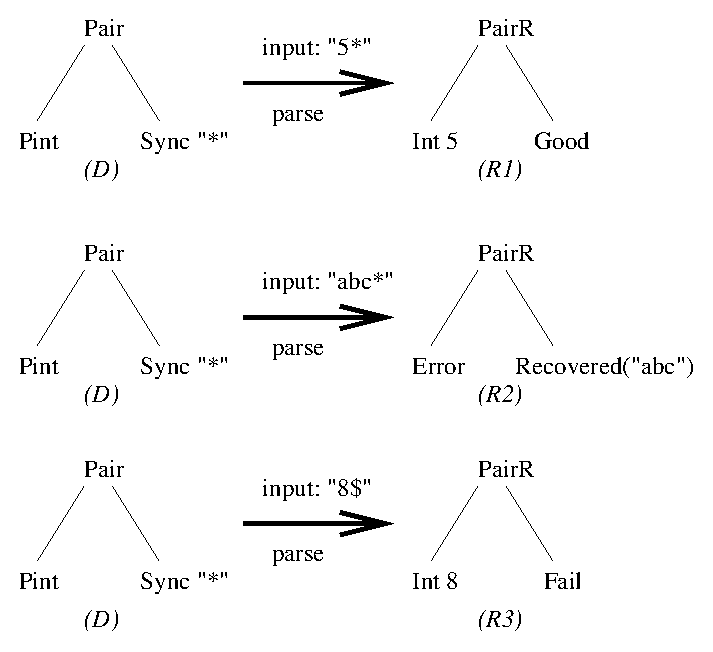
\includegraphics[width=0.8\columnwidth]{parse}
%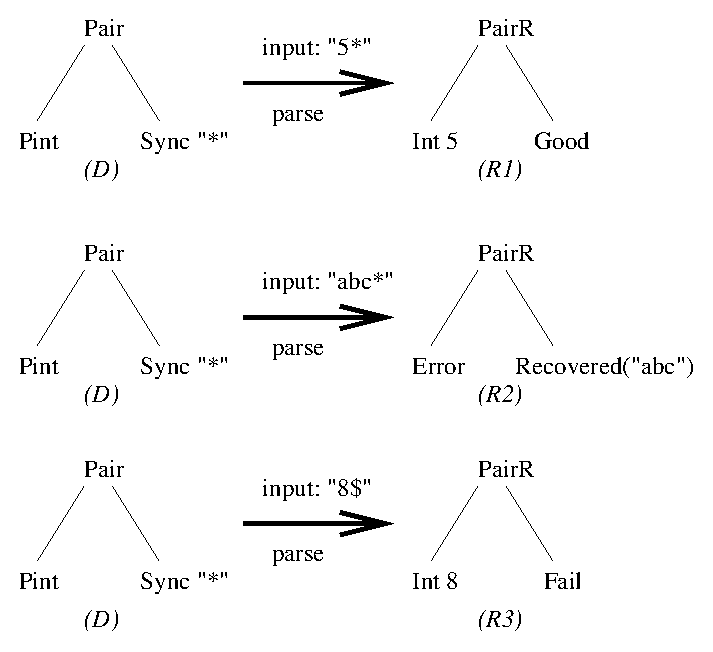
\epsfig{file=parse.eps, width=0.8\columnwidth}
\caption{Result of parsing three input lines}\label{fig:parse}
\end{center}
\end{figure}

\begin{figure*}[t]
\begin{center}
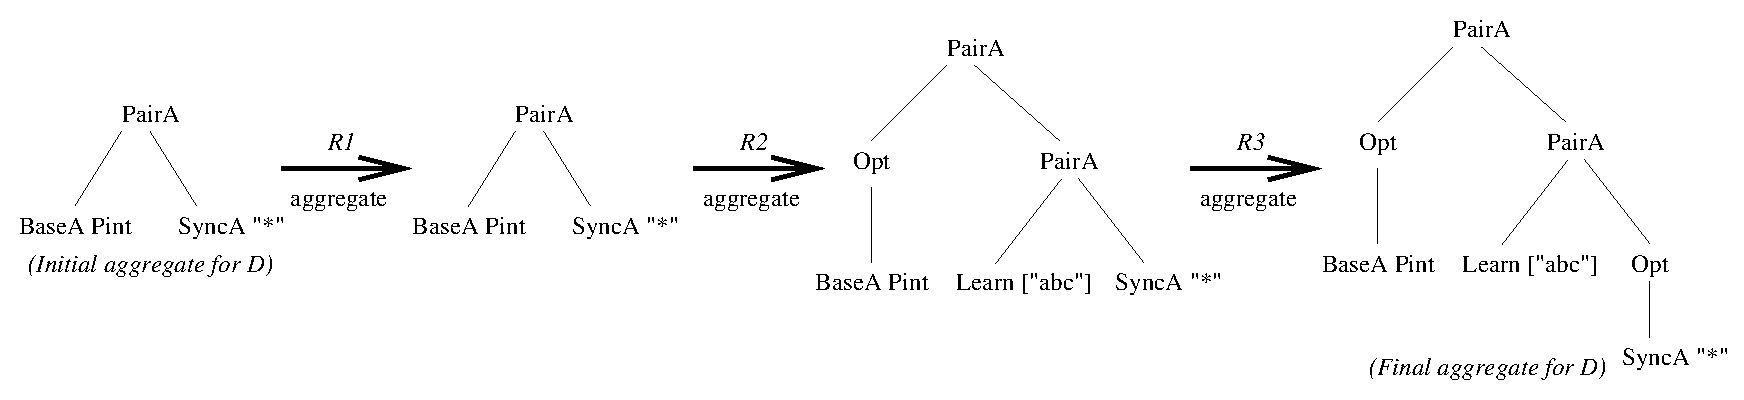
\includegraphics[width=2\columnwidth]{aggregate}
%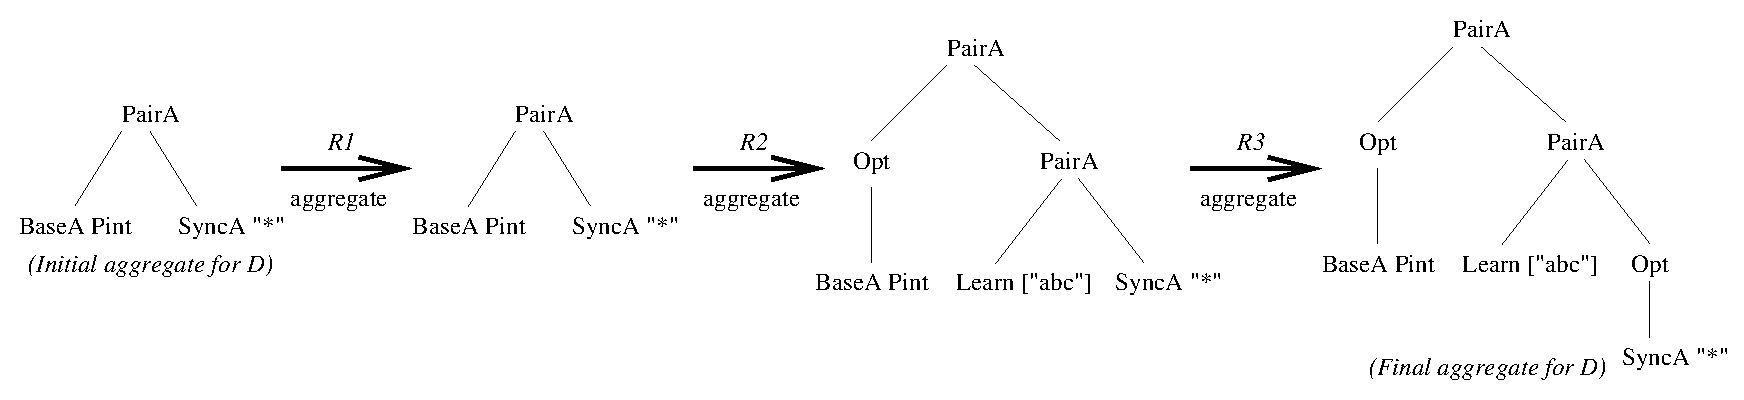
\epsfig{file=aggregate.eps, width=2\columnwidth}
\caption{Aggregation of three parses}\label{fig:aggregate}
\end{center}
\end{figure*}


%\begin{codebox}
%parse_all (d, x) =
%  switch (d) \{
%    case Pint =>  
%      (s, remainder) := match_prefix(x, "[0-9+\-]+");
%      if s != "" then return (Int s, remainder)
%      else return [(Error, x)];
%    case PstringME(re) => 
%      (s, remainder) := match_prefix(x, re);
%      if s != "" then return (Str s, remainder)
%      else return [(Error, x)];
%    case Sync s => 
%      (s', prefix, remainder) := match(x, s);
%      if s' = s and prefix = "" then return (Good, remainder)
%      elseif s' = "" then return (Fail, remainder)
%      else return [(Recovered prefix, remainder)]
%    case (x:d1, d2) =>
%      rs1 := parse_all (d1, x);
%      rs2 := [];
%      foreach (r1, remainder) in rs1 \{
%        (r2, remainder2) := parse_all (d2, remainder);
%        rs2 := rs2 + [((r1, r2), remainder2)]
%      \}
%    case (d1 + d2) => 
%	parse_all(d1, x) @ parse_all(d2, x)
%    case d array(sep, term) =>
%  \} 
%\end{codebox}    
%

\cut{%%%%%%%%%%%%%%%%%%%%%%%%%%%%%%%%

The {\tt parse\_all} function takes a description $d$ and an input string $x$, and returns
a list of all possible parses along with their respective ending position in the input. 
This function implements a standard recursive descent parser which recursively matches the
description structure (and sub-structures) with the input. To parse a pair $x: d_1 * d_2$, 
we first call {\tt parse\_all} on $d_1$ and get a list of parses. 
And then for each of the parse $r_1$ and corresponding end position, we bind $x$ to $r_1$ in
a private environment and  parse $d_2$ to get parses $l_2$. 
Finally for each parse $r_2$ in $l_2$ and each parse $r_1$ in $l_1$, 
construct a representation $(r_1, r_2)$, and return a list of all such pairs.
To parse a union $d_1 + d_2$, we simply return the concatenation of list of parses from
parsing $d_1$ and the list of parses from parsing $d_2$. To parse $d~ array(s, t)$,
we repeatedly attempt to parse $d$ until there's no more progress in the input.
And in each iteration, we also add parses generated from parsing $t$ as well, as if
the array has been terminated at this iteration. Figure \ref{fig:parse_base}
shows the {\tt parse\_base} function which parses a base token. The {\tt match\_prefix}
function matches the prefix of an input string with a regular expression and returns
the matched string and the remainder in the input. The {\tt match} function looks for
the first match of $s$ in input $x$, and returns the matched string $s'$, the prefix string
in $x$ before $s'$, and the remainder in the input.

\begin{figure}[t]
\begin{codebox}
parse_base (b, x) =
  switch (b) \{
  case Pint => 
    (s, suffix) := match_prefix(x, "[0-0+\-]+");
    if s <> "" then return [(Int s, suffix)];
    else return [(Error, x)]
  case PstringME(re) => 
    (s, suffix) := match_prefix(x, re);
    if s <> "" then return [(Str s, suffix)];
    else return [(Error, x)];
  case Sync s => 
    (s', prefix, remainder) := match(x, s);
    if s' = s and prefix = "" then 
      return (Good, remainder)
    elseif s' = "" then 
      return (Fail, remainder)
    else return [(Recovered prefix, remainder)]
  \}
\end{codebox}
\caption{Function to parse a base token or a sync token} \label{fig:parse_base}
\end{figure}

As an example, let $d$ be {\tt (Pint, Sync "|") + (PstringME "[a-z]+", Sync "|")}, 
and $x$ be ``\verb#abc|#''. {\tt parse\_all(d, x)} gives the following two possible parses:
{\small
\begin{verbatim}
  inl (Error, Recovered "abc")
  inr (Str "abc", Good)
\end{verbatim}
}

The {\tt aggregate} function adds a parse into an existing aggregate structure. When there is
no errors in the parse, it makes no changes to the aggregate. If the parse contains 
an error or failure for parsing token $b$, then the aggregate component 
$b$ is transformed to $opt~ b$, to indicate that $b$ node is optional. 
If a parse contains a recovered data $Recovered~ r$, then
a optional learn node will be created before the sync node. And the new aggregate component will be
$(opt (l [r]),~ Sync~ s)$. If the aggregate structure already contains the learn node before this
sync node, then recovered data $r$ will be added to the list under $l$.


}%%%%%%%%%%%%%%%%%%%%%%%%%%%%%%%%% END OF CUT %%%%%%%%%%%%%%%%

% - problem definition (as close to the previous description as possible) (but we don't
%   have a metric to measure how close yet, do we want to mention tree edit distance??)
% - overview of algorithm: parsing + aggregating + rewriting
% - parsing algo (parse rep, score metric, pseudo-code)
% - aggregating algo (in pseudo code)
% - selection of top aggregates
% - update original description
% - rewriting rules (data independent, data dependent, OptsTable)


\subsection{Description Rewriting}
Once we have successfully parsed, aggregated and relearned a new
chunk of data, we optimize the new description using rewriting rules.  
Our original non-incremental
algorithm already had such an optimization
phase; we have modified and tuned the algorithm for use in
the incremental system.

Description rewriting is based on optimizing an information-theoretic
Minimum Description Length (MDL) score~\cite{mdlbook}, which is 
defined over descriptions
\cd{D} as:
\[\mbox{\rm{MDL}(\texttt{D})} = \costdescription{D} + w \times \acostdata{D}{x_1, \ldots, x_k},\]
where $\costdescription{D}$ is called the {\em type complexity} of \cd{D}
and \\
$\acostdata{D}{x_1, \ldots, x_k}$ is called the {\em atomic data 
complexity}.  The type complexity is a measure of the size of the 
abstract syntax of \cd{D}.  The atomic data 
complexity of data records $x_1, \ldots, x_k$ relative to \cd{D} 
is the number of bits required
to transmit an {\em average} data record given the description \cd{D}.
The MDL score of \cd{D} is the weighted sum of these two components.  
Our experiments indicate a weight $w$ of approximately 10 is effective
in our domain.

Given a rewriting rule that rewrites \cd{D} to \cd{D'}, the
rule fires if and only if \rm{MDL}(\texttt{D}) $\leq$ \rm{MDL}(\texttt{D'}).
Rewriting continues until no further rule can fire.
Hence, our rewriting strategy is a greedy local
search.

\begin{figure}[t]
\begin{center}
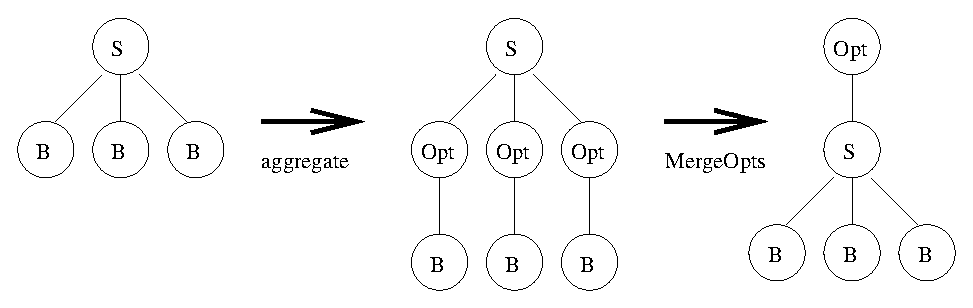
\includegraphics[width=\columnwidth]{opts}
%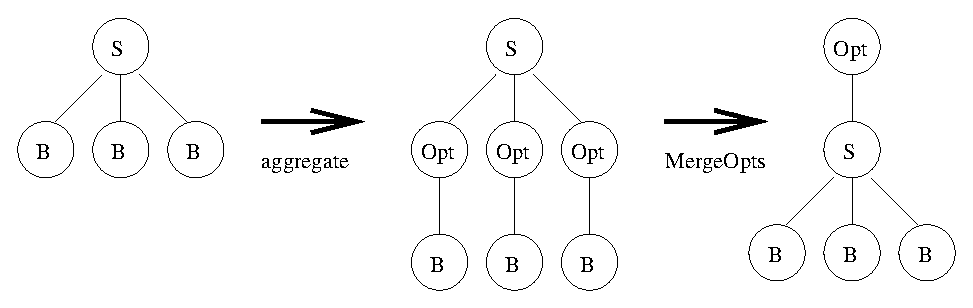
\epsfig{file=opts.eps,width=\columnwidth}
\caption{MergeOpts rewriting rule}\label{fig:opts}
\end{center}
\vskip -2ex
\end{figure}

%% When the incremental learning algorithm produces a refined description
%% from an aggregate, the algorithm applies rewriting rules
%% to the new description to improve its quality and readability.
%% Most of the rules are data-independent and inherited from \learnpads{}, such as 
%% removing degenerate lists and flattening nested structs and unions.

The original learning system contains many MDL-based rewriting rules, for example,
to flatten nested structs and unions and
to refine ranged types.
{\em BlobFinding} is an important new rewriting rule. 
This rule takes a given sub-description \cd{D} and uses a heuristic to 
determine if the type complexity of \cd{D} is too high relative to the amount of data it covers.
The heuristic is that if the height of \cd{D} is larger than \cd{minBlobHeight}
(which is empirically determined), and there is an identifiable constant string 
or pattern \cd{re} that immediately follows
\cd{D}, then we rewrite \cd{D} to 
\cd{Pstring\_SE(:re:)}.
Description \cd{Pstring\_SE} is a \pads{} base type that is similar to \cd{Pstring},
except it uses a stopping regular pattern as opposed to a stopping character
to indicate termination. This rule is tremendously helpful
in controlling the size and
complexity of learned descriptions.  Without it, descriptions can
grow in complexity to the point where parsing is slow and the algorithm fails to scale.


We also introduced a new {\em data dependent} rewriting rule called {\em MergeOpts}
to optimize a pattern that occurs frequently in descriptions during incremental
learning.  Recall that the aggregate function
introduces \cd{Opt} nodes above a \cd{BaseA} or \cd{SyncA} node 
whenever the corresponding \cd{Base} or \cd{Sync} token in 
the description failed to 
parse. When faced with an entirely new form of data, 
the algorithm is likely to introduce a series of \cd{Opt} nodes as
each type in the original description fails in succession. 
The {\em MergeOpts} rule collapses these consecutive \cd{Opt} nodes if they
are correlated, \ie{}, either they are all always present or all always
absent.  To verify this correlation, the algorithm maintains a
table that records the branching decisions when parsing each
data line. It uses this table to determine whether to merge
adjacent \cd{Opt} nodes during rewriting. 
\figref{fig:opts} illustrates the effect of this rule.  In the figure,
$S$ denotes a struct and $B$ a base token.

\vspace{20pt}
